% !TEX root = main.tex

% TODO:
% REMARK:

\section{ Systematic Uncertainty}
\label{sec:Systematic}

	Besides the statistical uncertainty, there are also some systematic uncertainty from detector's issue, reconstruction procedure, simulating process...etc. In this snalysis, the primary systematic uncertainties are from the simulation correction. 

	\subsection{Introduction of systematic uncertainty}
	\label{ssec:Syst_type}
		\subsubsection{Pileup re-weighting}
		\label{sssec:Syst_PU}

			% https://twiki.cern.ch/twiki/bin/viewauth/CMS/PileupMCReweightingUtilities?fbclid=IwAR0SuZFQ5Um0IfZn1-CHXia6NPMYe2_7cz2OGXxhCYvNvfl_tTBke-w22l8

			Since the pileup performance under data and simulation(MC) have discrepancy, there is MC reweighing of pileup in any events which is mentioned in section.\ref{sssec:DataAndMC_PU}. However, there is also an uncertainty of pileup reweight. The pp inelastic scattering cross section is used to calculate the pileup distribution and then used to implement the pileup reweight, so this cross section has its mean value and uncertainty 69.2$mb^{-1}$ $\pm$5\%. Then the pileup reweighing factor may be affected by this cross section as the pileup reweighting systematic uncertainty.

		\subsubsection{Jet energy correction and resolution}
		\label{sssec:Syst_JECJER}

			The JER and JEC are mentioned in section.\ref{ssec:PhysObj_jet}, they might have shifted or smeared the energy spectrum of any reconstructed jets. That is to say, the four-momentum, invariant mass, and also $p_T$ would be affected by the adoption of JEC and JER, and the uncertainty of them would fluctuate the kinematics also affect the results of object and event selection. The correctly application of one standard deviation uncertainty of JEC and JER could cover the jet reconstruction issues also the uncertainty of MET($E_T^{miss}$, missing $E_T$).
			

		\subsubsection{b-tagged scale factor}
		\label{sssec:Syst_btag}

			When applying the btagging reweight on each event, the btagging scale factors are included in the weight measurement(Eq.\ref{eq:btag_weight_2}). The scale factors were calculated by BTV POG, and there are the scale factors values and uncertainty being obtained from them. Therefore, the uncertainty would propagate from btagging scale factors to the btagging weight, and the uncertainty can be implemented by the weight.

		\subsubsection{Lepton identification, isolation, reconstruction and trigger efficiencies}
		\label{sssec:Syst_lepsf}

			The lepton identification, isolation, reconstruction and trigger scale factors were mentioned in section.\ref{sssec:DataAndMC_LepEffSF}. The event with specific(under corresponding $p_T$, $\eta$ values) selected lepton should be corrected by scale factor on the weight of this event. However, the scale factors are also calculated from POG with real data and simulation, so there must be uncertainty on each scale factor which is each bin's value of Fig.\ref{DataMC:fig:lepsf}.

	\subsection{Implementation and results}
	\label{ssec:Syst_imp_result}

		The approaches to apply the systematic uncertainty are shown below. This is expected to use 5000 pseudo data set to calculate the systematic uncertainty of $A'_{cp}$. We nneed to use the real dataset's $M_{lb}$-$A_{cp}(O_i)$ distribution(2D) to generate 5000 sets of pseudo dataset. The generated method is by Monte Carlo algorithm and adopted with yields from poisson distribution with mean is real dataset's yields. For example, Fig.\ref{Syst:fig:PD} is one of the generated pseudo dataset under $M_{lb}$-$O_{6}$ in muon channel(MVA reconstruction result). 

		\begin{figure}[H]
		\centering
			\subfigure[one of pseudo dataset of $M_{lb}$-$O_6$ (muon channel)]{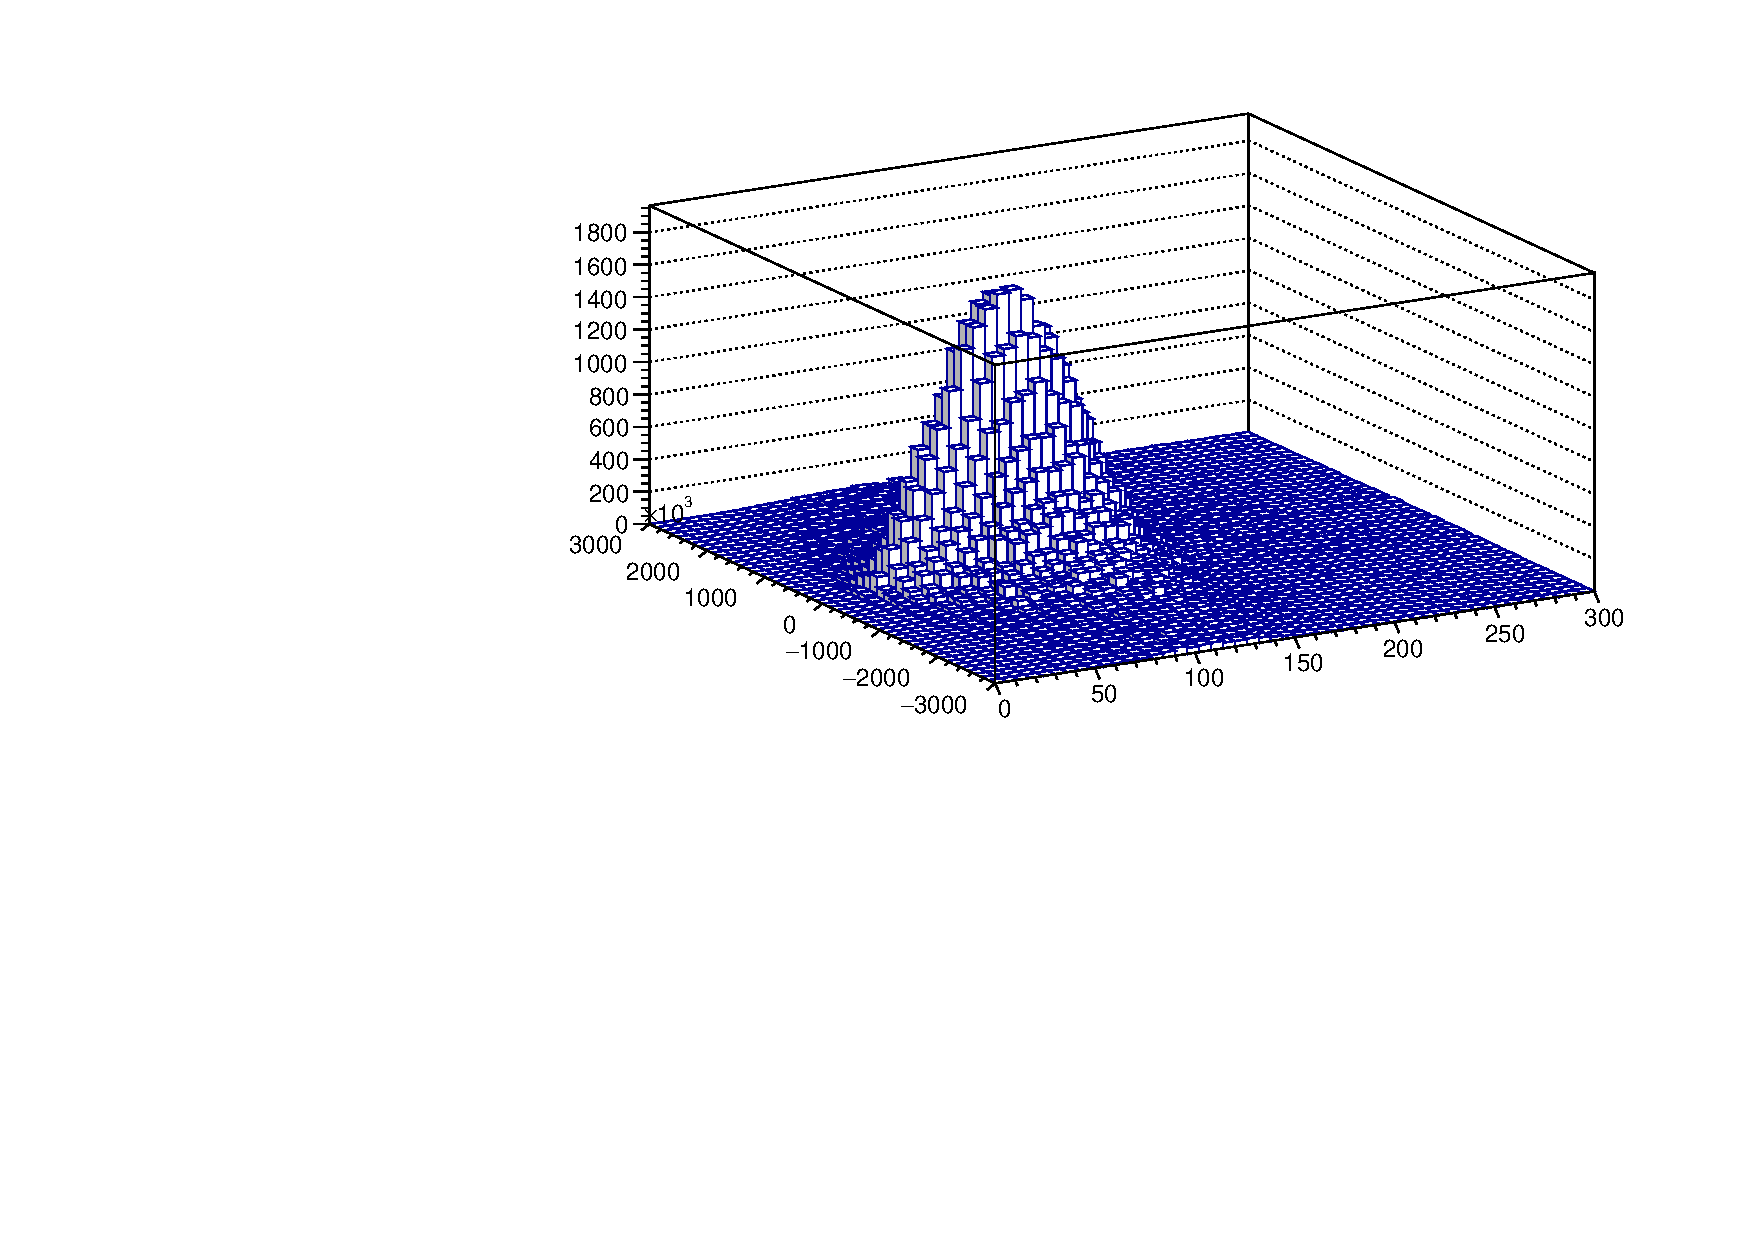
\includegraphics[width=0.65\textwidth]{Figures/SystUnc/PD_nominal_O6_mu.pdf}}\\
		\caption{Generated pseudo dataset ($M_{lb}$-$O_6$ in muon channel ($M_{lb}$:[0,300],$O_i$:[-3000,3000])}
		\label{Syst:fig:PD}
		\end{figure}
		\FloatBarrier

		For each pseudo dataset, we have a series of implementation -- The illustration of systematice implementation is shown below in Fig.\ref{Syst:fig:approach}. First, we applied the one standard deviation systematic uncertainty of one kind of systematic on the signal simulation sample, then do full selection on it to get the signal template under $M_{lb}$ with systematic uncertainy. For instance, the Fig.\ref{Syst:fig:template} shows the signal template without any systematic uncertainty(nominal), the signal template with JER(+1$\sigma$) systematic uncertainty and the original background template.

		\begin{figure}[H]
		\centering
			\subfigure[Nominal signal template]{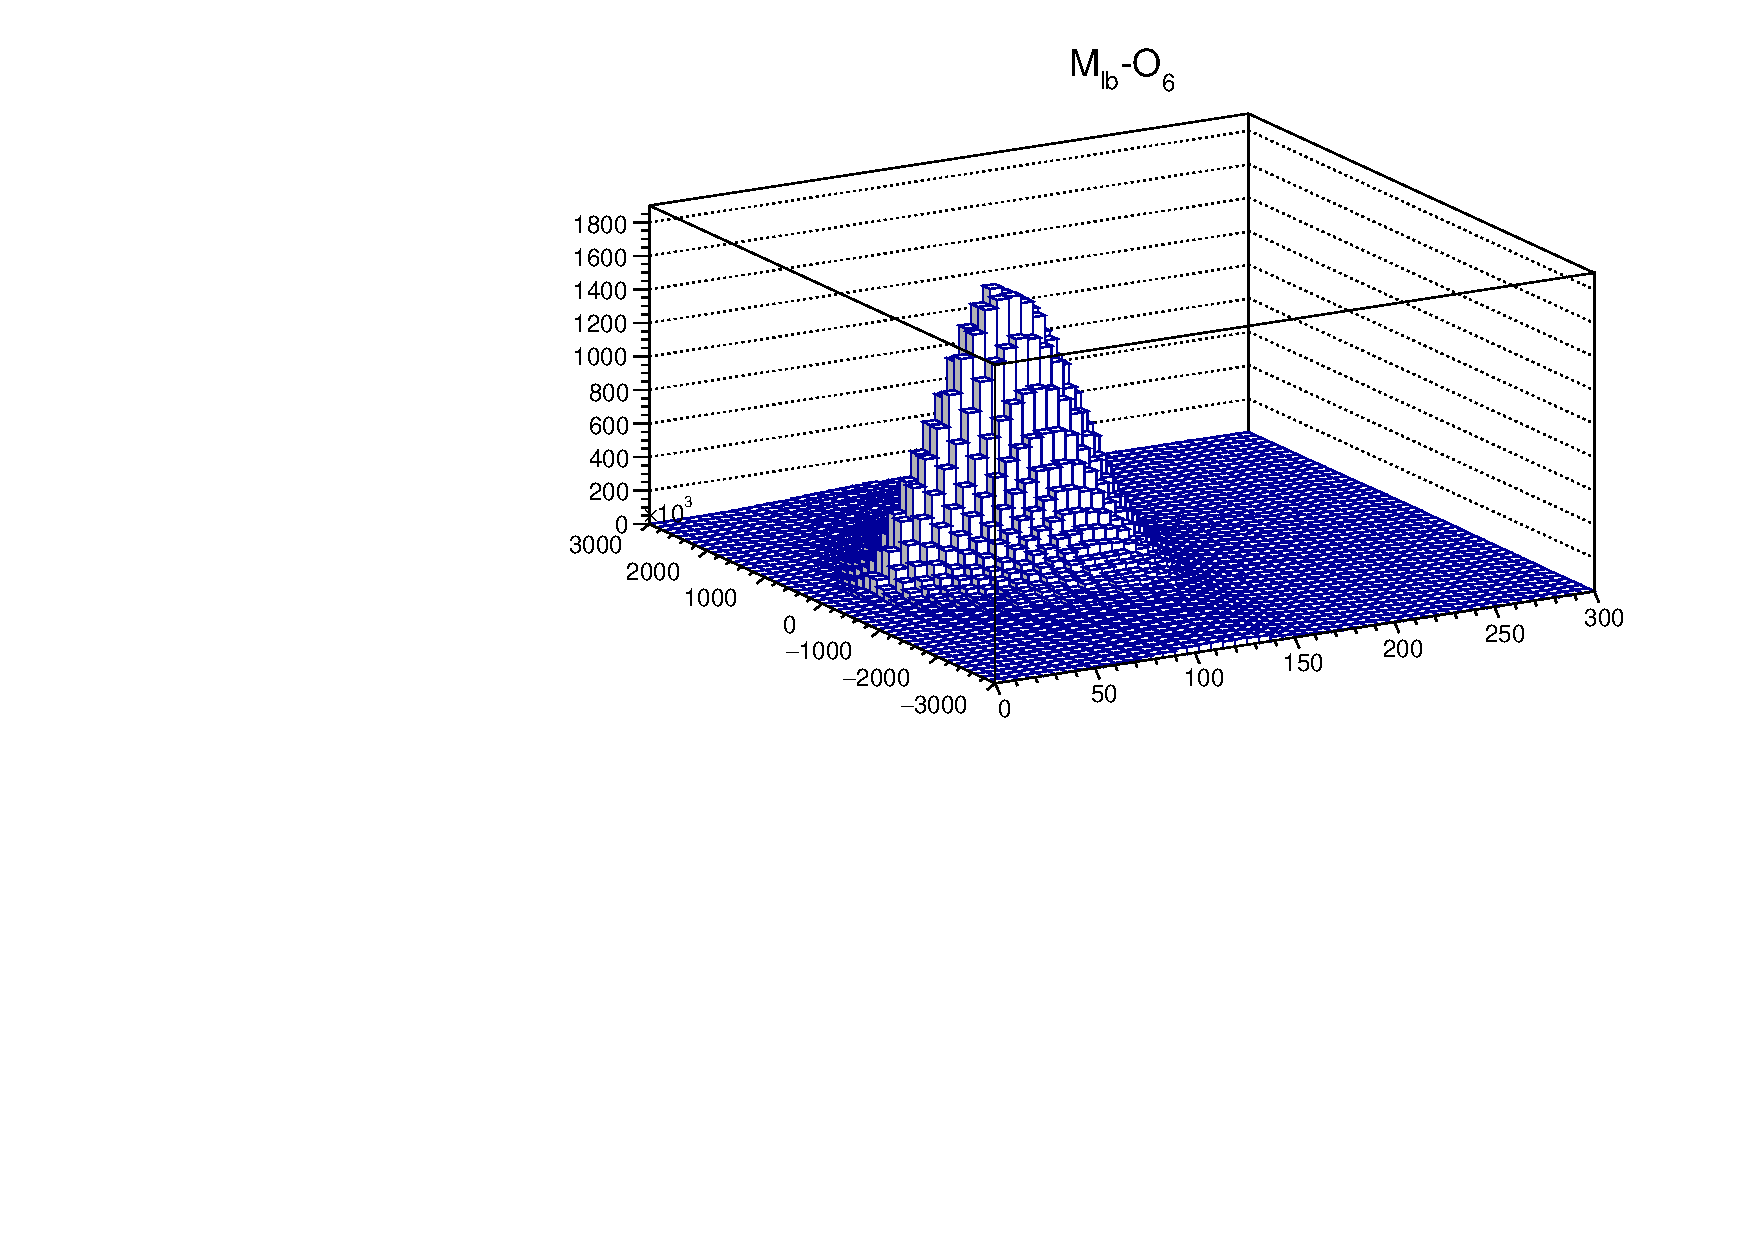
\includegraphics[width=0.45\textwidth]{Figures/SystUnc/nominal_O6_mu_template.pdf}}
		    \subfigure[JER +1$\sigma$ signal template]{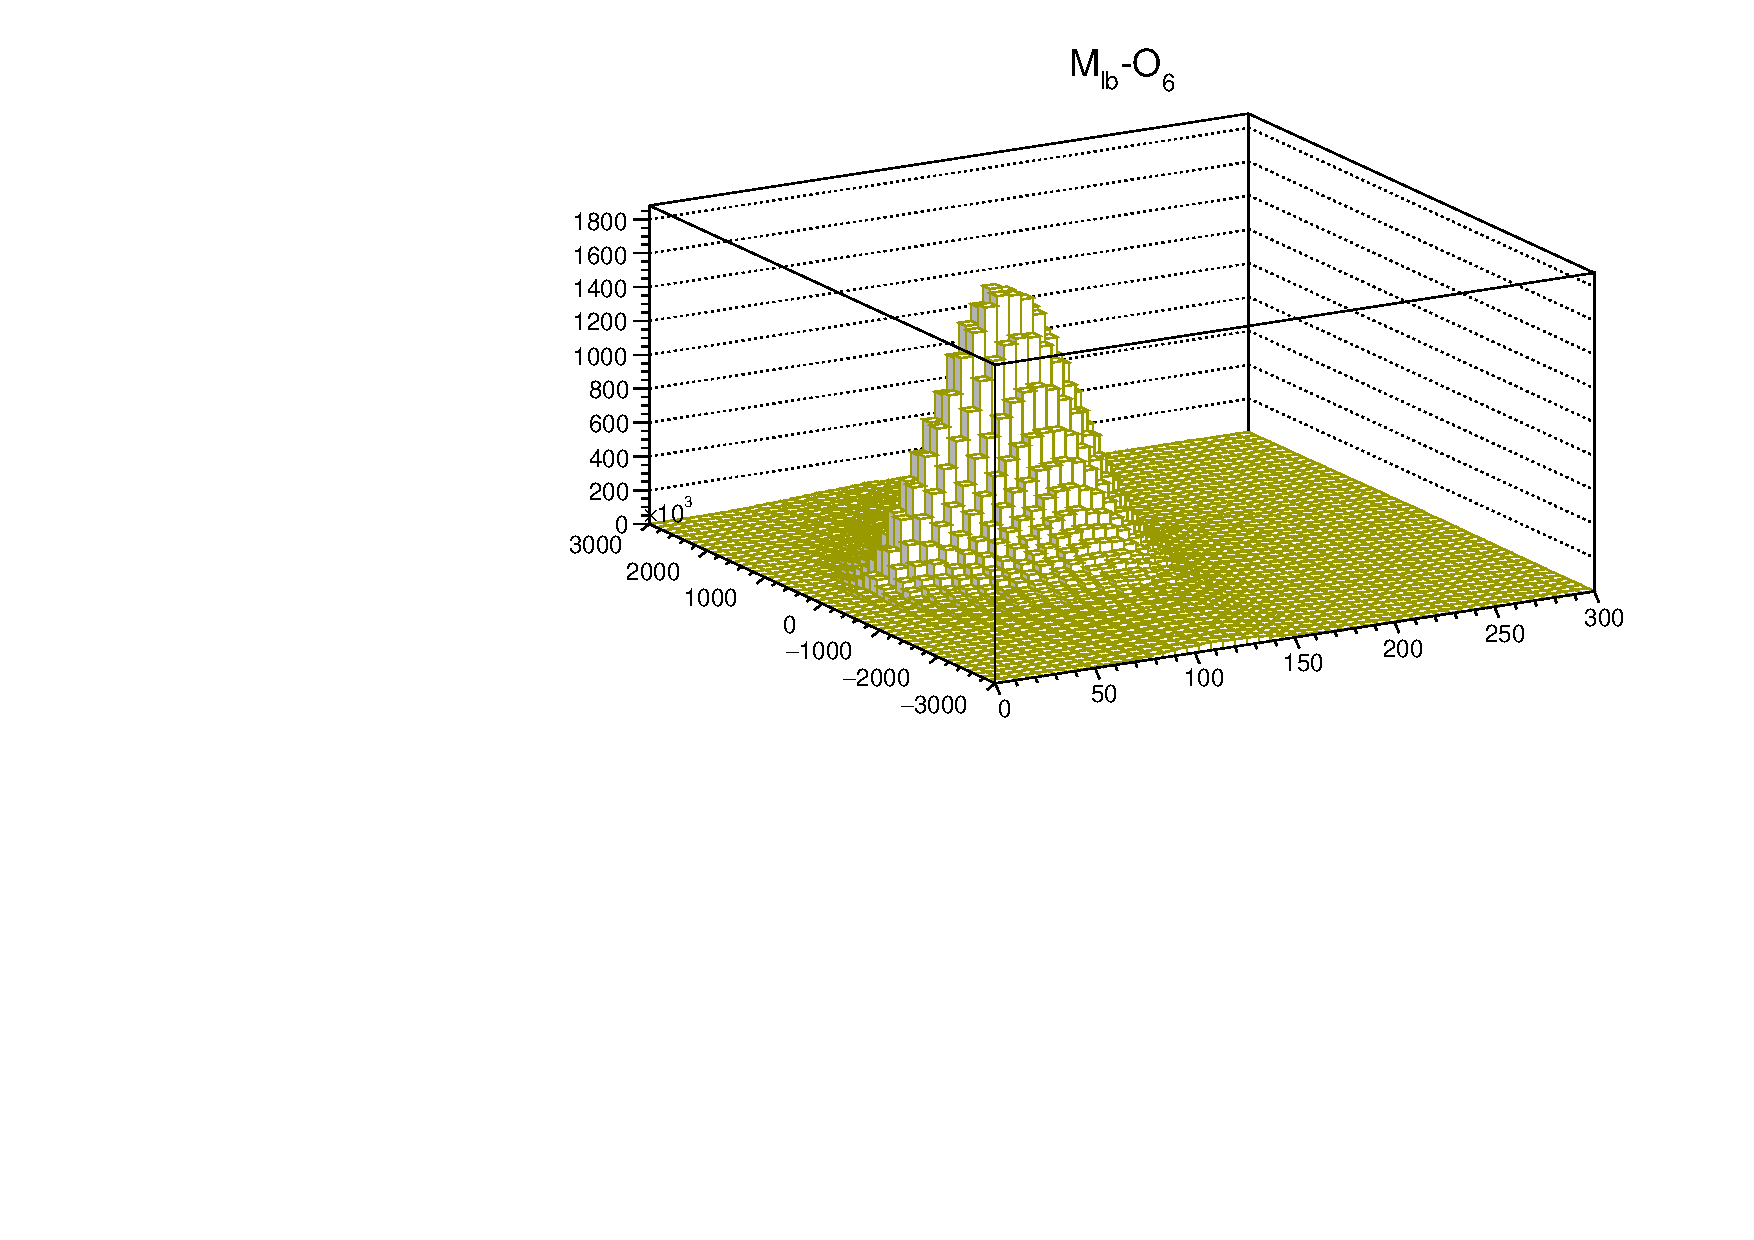
\includegraphics[width=0.45\textwidth]{Figures/SystUnc/JERup_O6_mu_template.pdf}}\\
		    \subfigure[Background template]{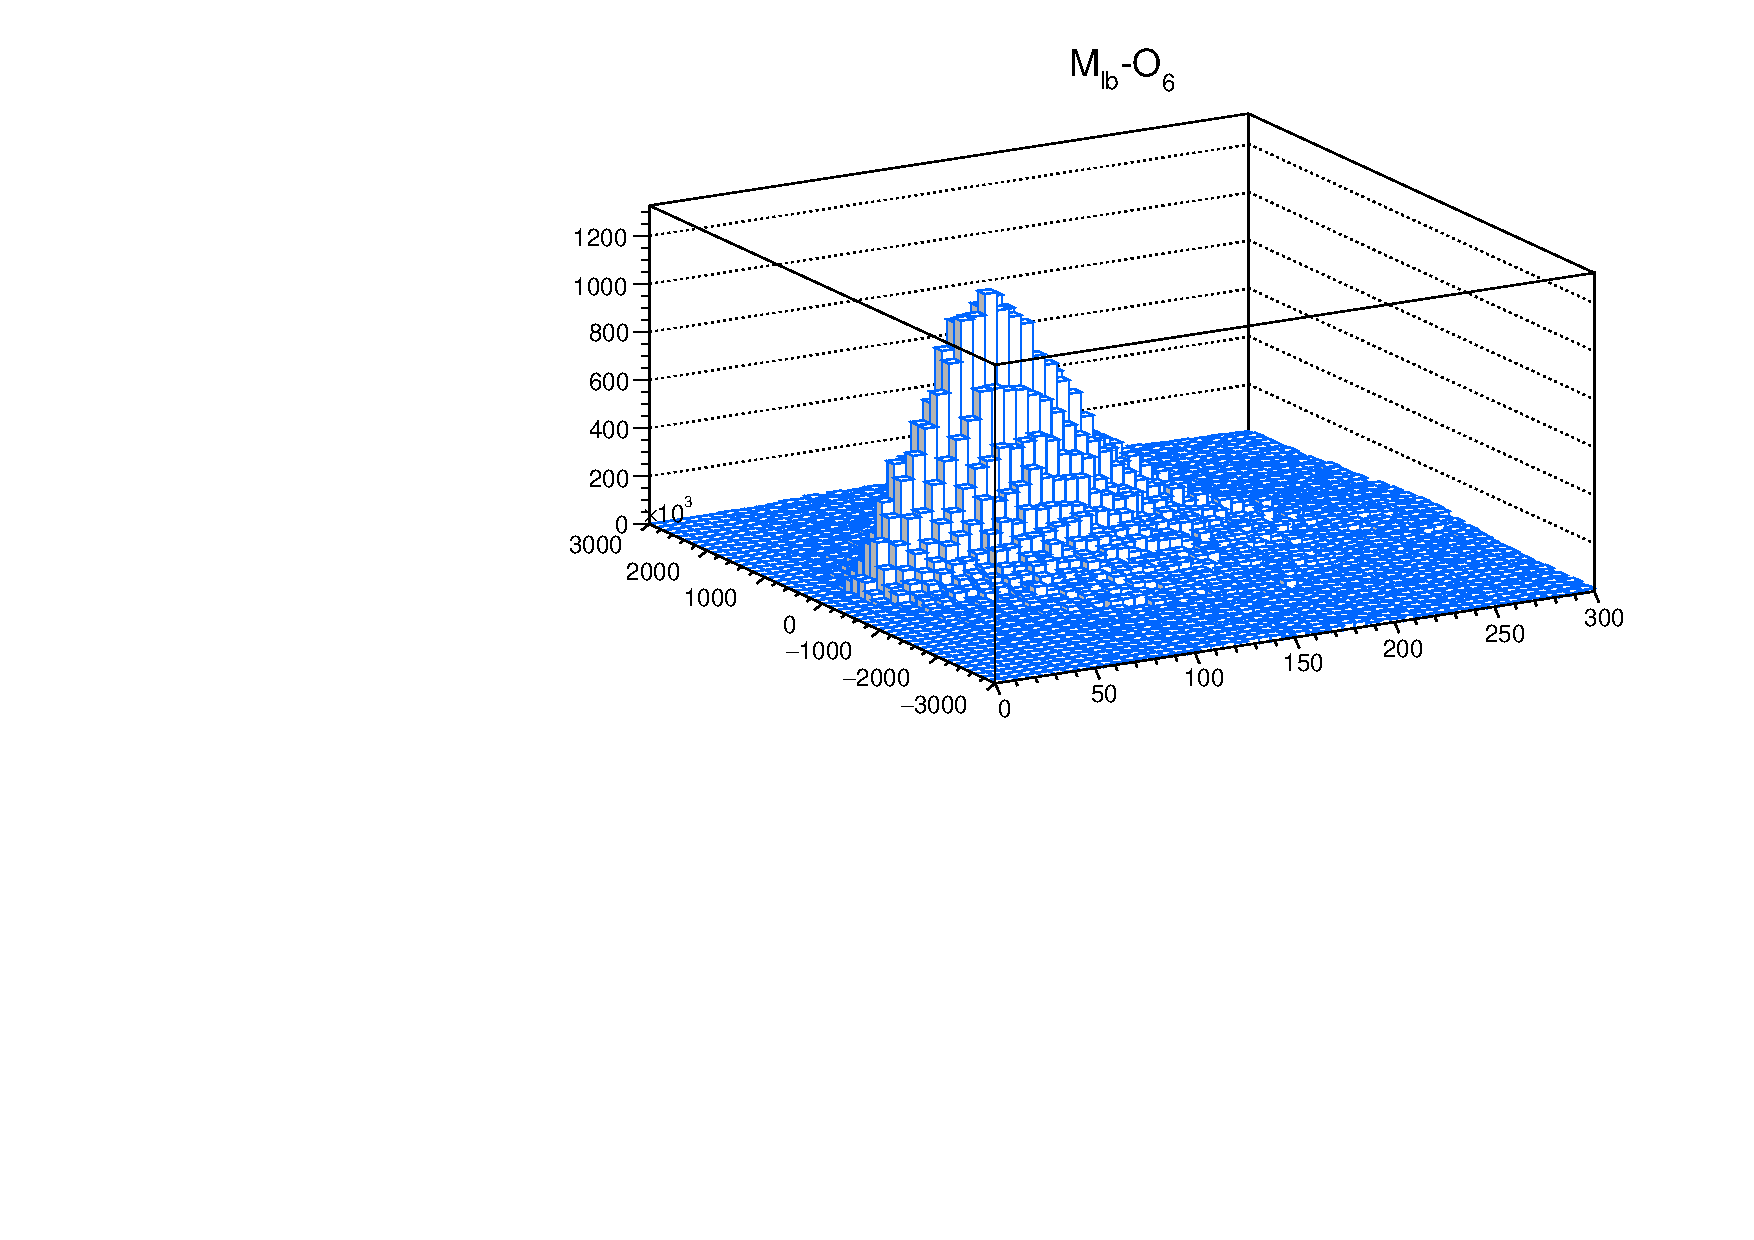
\includegraphics[width=0.45\textwidth]{Figures/SystUnc/nominal_bkg_O6_mu_template.pdf}}
		\caption{Nominal signal template, JER +1$\sigma$ signal template, and background template in muon channel}
		\label{Syst:fig:template}
		\end{figure}
		\FloatBarrier

		Secondly, by using this signal template and original background template to do the background subtraction(section.\ref{ssec:bkg_sub} and Fig.\ref{BkgEst:fig:Bkt_sub}) and get the $A'_{cp}$(of observable $O_i$) with systematic uncertainty. Lastly, we get the $A'_{cp}$ of nominal version(without any systematic uncertainty) and systematic uncertainty version and their $\Delta A'_{cp}$ would be got.

		\begin{figure}[H]
		\centering{}
	    	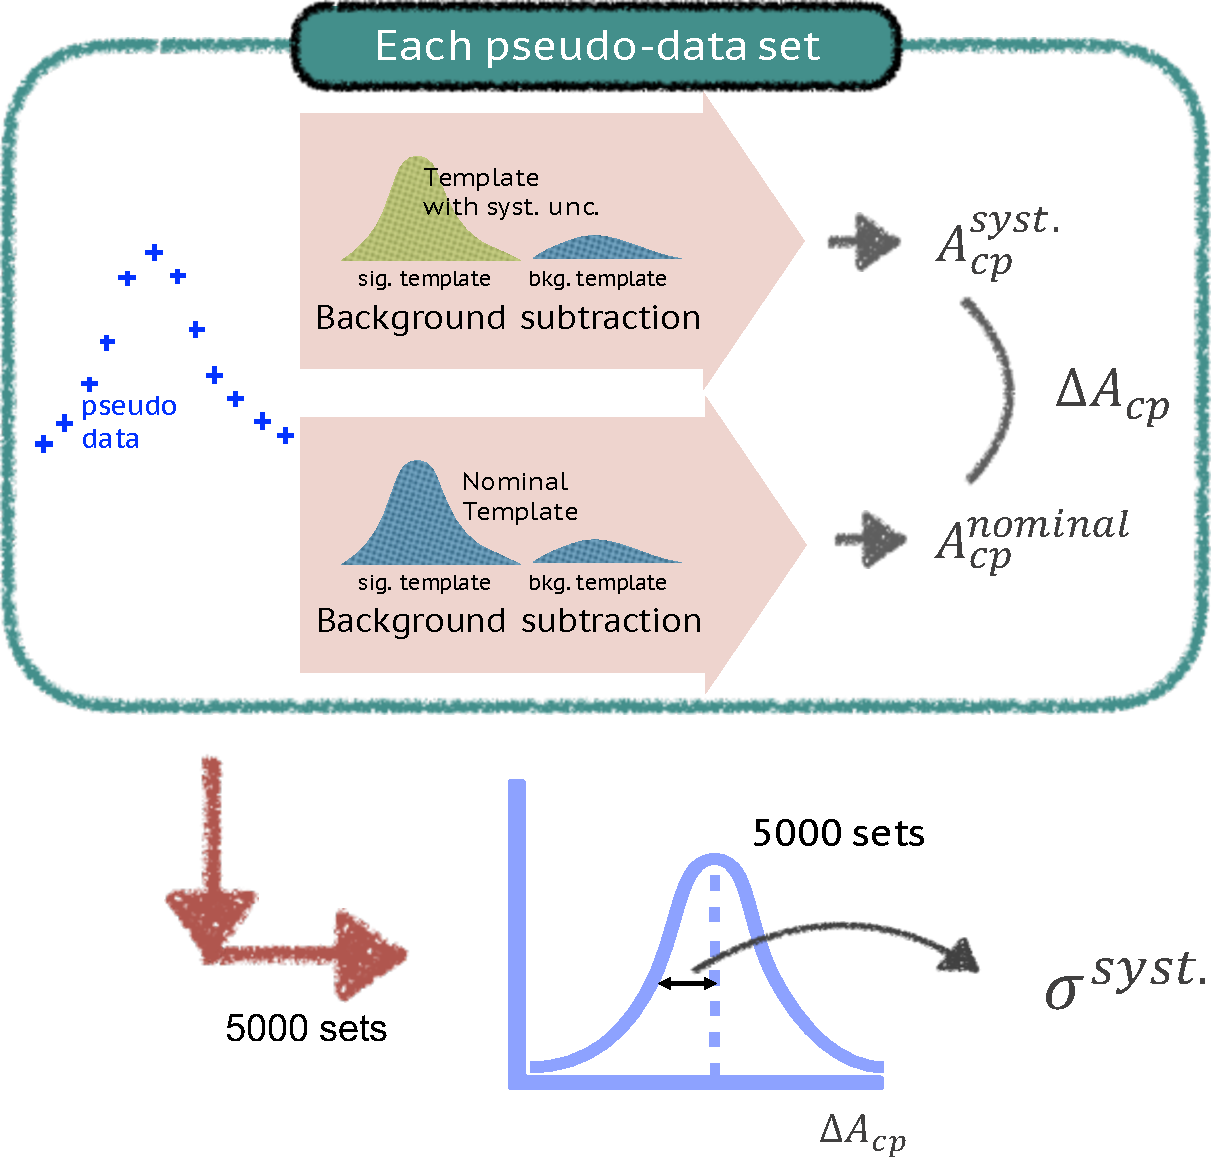
\includegraphics[width=0.85\textwidth]{Figures/SystUnc/approach_syst.pdf}\\
		\caption{Process of measuring systematic uncertainty}
		\label{Syst:fig:approach}
		\end{figure}
		\FloatBarrier

		We repeat the previous procedure on 5000 pseudo dataset and get a collection of 5000 $\Delta A'_{cp}$ and their gathering distribution. The mean value of the distribution may be the final systematic uncertainty of the $A'_{cp}$, however, in this analysis, we consider the standard deviation of the distribution as the absolute value of systematic uncertainty, and the mean value could be used to decide the positive or negative sign of systematic uncertainty. In the process, the fitted signal/background yields in 5000 sets of pseudo dataset could be obviously differ between nominal case and systematic case. Futhermore, the fitted signal/background $\Delta$yields distribution and $\Delta A'_{cp}$ distribution between nominal and systematic cases could be fitted by a gaussian distribution. There are the example of fitted signal/background $\Delta$yields distribution(Fig.\ref{Syst:fig:deviation_sig}, \ref{Syst:fig:deviation_bkg}) and $\Delta A'_{cp}$ distribution(Fig.\ref{Syst:fig:deviation_Acp}) of JER(+1$\sigma$) systematic uncertainty of $O_6$ in muon channel.


		\begin{figure}[H]
		\centering
		    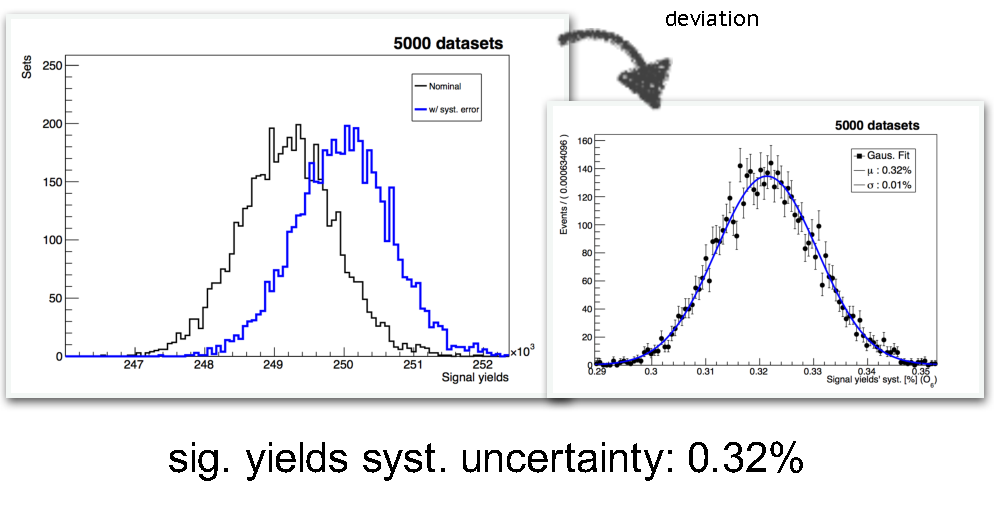
\includegraphics[width=0.75\textwidth]{Figures/SystUnc/sig_yields_unc.pdf}\\
		\caption{Signal yields distribution and $\Delta$ signal yields distribution (Nominal and JER(+1$\sigma$) $O_6$ muon channel case) }
		\label{Syst:fig:deviation_sig}
		\end{figure}
		\FloatBarrier

		\begin{figure}[H]
		\centering
		    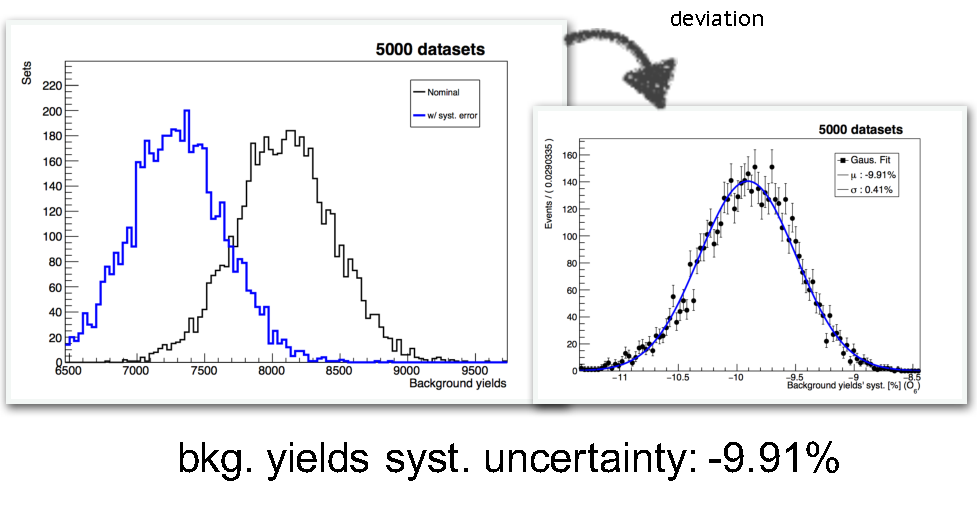
\includegraphics[width=0.75\textwidth]{Figures/SystUnc/bkg_yields_unc.pdf}\\
		\caption{Background yields distribution and $\Delta$ background yields distribution (Nominal and JER(+1$\sigma$) $O_6$ muon channel case) }
		\label{Syst:fig:deviation_bkg}
		\end{figure}
		\FloatBarrier

		\begin{figure}[H]
		\centering
		    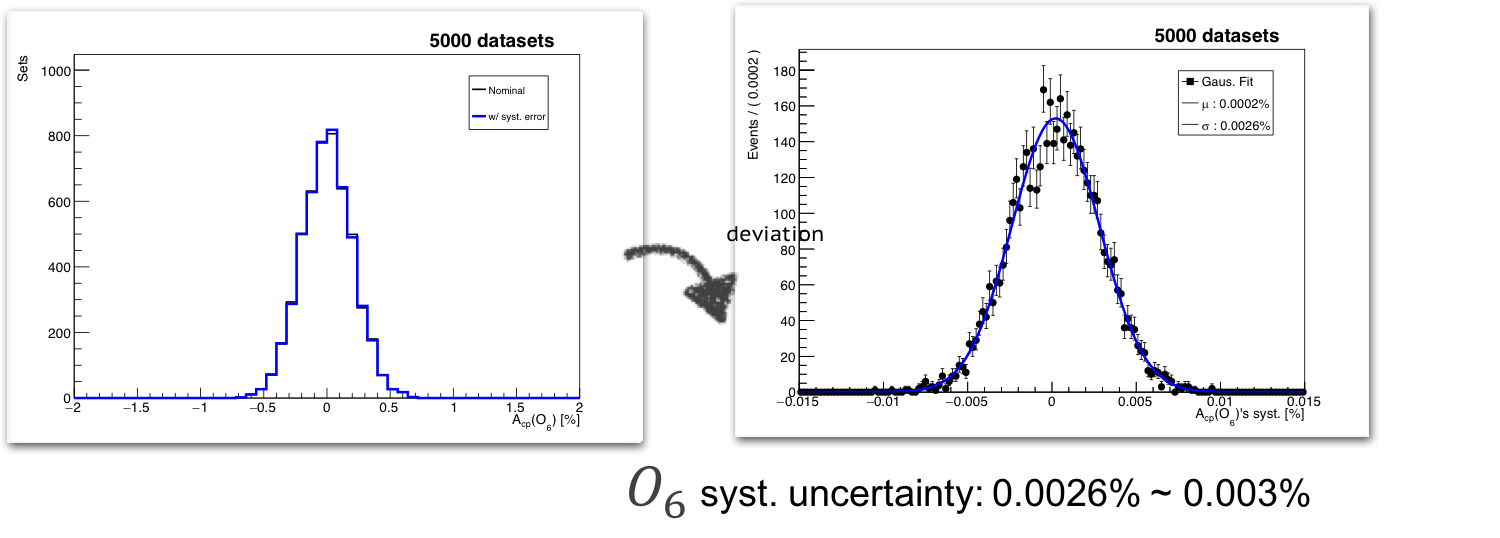
\includegraphics[width=0.95\textwidth]{Figures/SystUnc/Acp_unc.png}\\
		\caption{$A'_{cp}$ distribution and $\Delta A'_{cp}$ distribution (Nominal and JER(+1$\sigma$) $O_6$ muon channel case) }
		\label{Syst:fig:deviation_Acp}
		\end{figure}
		\FloatBarrier

		The following tables are the result of systematic uncertainty in both muon channel and electron channel.

		\begin{center}
		\setlength{\tabcolsep}{12pt}
		\begin{longtable}{ | c | c c c c | }
		\caption{Systematic of $A_{cp}(O_i)$ in Muon channel [\%] ($\chi^2_{min}$)}\\
		\hline
		 [\%] & $O_3$ & $O_6$ & $O_{12}$ & $O_{14}$ \\
		\hline
		b-tagging($+1\sigma$) & 0.002 & 0.002 & 0.002 & -0.002 \\
		b-tagging($-1\sigma$) & -0.002 & -0.002 & -0.002 & 0.002 \\
		\hline
		Pileup($+1\sigma$) & 0.001 & 0.001 & 0.001 & -0.001 \\
		Pileup($-1\sigma$) & -0.001 & -0.001 & -0.001 & 0.001 \\
		\hline
		Lepton($+1\sigma$) & 0.000 & 0.000 & 0.000 & -0.000 \\
		Lepton($-1\sigma$) & -0.000 & -0.000 & -0.000 & 0.000 \\
		\hline
		JER($+1\sigma$) & 0.006 & 0.005 & 0.005 & -0.006 \\
		JER($-1\sigma$) & -0.006 & -0.006 & -0.006 & 0.006 \\
		\hline
		JEC($+1\sigma$) & 0.006 & 0.006 & 0.006 & -0.006 \\
		JEC($-1\sigma$) & -0.006 & -0.006 & -0.006 & 0.006 \\
		\hline
		\end{longtable}
		\end{center}

		\begin{center}
		\setlength{\tabcolsep}{12pt}
		\begin{longtable}{ | c | c c c c | }
		\caption{Systematic of $A_{cp}(O_i)$ in Electron channel [\%] ($\chi^2_{min}$)}\\
		\hline
		 [\%] & $O_3$ & $O_6$ & $O_{12}$ & $O_{14}$ \\
		\hline
		b-tagging($+1\sigma$) & -0.002 & -0.002 & -0.002 & 0.002 \\
		b-tagging($-1\sigma$) & 0.002 & 0.002 & 0.002 & -0.002 \\
		\hline
		Pileup($+1\sigma$) & -0.001 & -0.001 & -0.001 & 0.001 \\
		Pileup($-1\sigma$) & 0.001 & 0.001 & 0.001 & -0.001 \\
		\hline
		Lepton($+1\sigma$) & -0.000 & -0.000 & -0.000 & 0.000 \\
		Lepton($-1\sigma$) & 0.000 & 0.000 & 0.000 & -0.000 \\
		\hline
		JER($+1\sigma$) & -0.008 & -0.008 & -0.008 & 0.008 \\
		JER($-1\sigma$) & 0.008 & 0.007 & 0.008 & -0.007 \\
		\hline
		JEC($+1\sigma$) & -0.008 & -0.008 & -0.008 & 0.008 \\
		JEC($-1\sigma$) & 0.007 & 0.007 & 0.007 & -0.007 \\
		\hline
		\end{longtable}
		\end{center}

		\begin{center}
		\setlength{\tabcolsep}{12pt}
		\begin{longtable}{ | c | c c c c | }
		\caption{Systematic of $A_{cp}(O_i)$ in Muon channel [\%] (MVA-A)}\\
		\hline
		 [\%] & $O_3$ & $O_6$ & $O_{12}$ & $O_{14}$ \\
		\hline
		b-tagging($+1\sigma$) & -0.002 & 0.002 & -0.002 & 0.002 \\
		b-tagging($-1\sigma$) & 0.002 & -0.002 & 0.002 & -0.002 \\
		\hline
		Pileup($+1\sigma$) & -0.001 & 0.001 & -0.001 & 0.001 \\
		Pileup($-1\sigma$) & 0.001 & -0.001 & 0.001 & -0.001 \\
		\hline
		Lepton($+1\sigma$) & -0.000 & 0.000 & -0.000 & 0.000 \\
		Lepton($-1\sigma$) & 0.000 & -0.000 & 0.000 & -0.000 \\
		\hline
		JER($+1\sigma$) & -0.003 & 0.003 & -0.003 & 0.003 \\
		JER($-1\sigma$) & 0.002 & -0.002 & 0.002 & -0.002 \\
		\hline
		JEC($+1\sigma$) & -0.003 & 0.003 & -0.003 & -0.003 \\
		JEC($-1\sigma$) & 0.003 & -0.003 & 0.003 & 0.003 \\
		\hline
		\end{longtable}
		\end{center}

		\begin{center}
		\setlength{\tabcolsep}{12pt}
		\begin{longtable}{ | c | c c c c | }
		\caption{Systematic of $A_{cp}(O_i)$ in Electron channel [\%] (MVA-A)}\\
		\hline
		 [\%] & $O_3$ & $O_6$ & $O_{12}$ & $O_{14}$ \\
		\hline
		b-tagging($+1\sigma$) & 0.002 & -0.002 & -0.002 & 0.002 \\
		b-tagging($-1\sigma$) & -0.002 & 0.002 & 0.002 & -0.002 \\
		\hline
		Pileup($+1\sigma$) & 0.001 & -0.001 & -0.001 & 0.001 \\
		Pileup($-1\sigma$) & -0.001 & 0.001 & 0.001 & -0.001 \\
		\hline
		Lepton($+1\sigma$) & 0.000 & -0.000 & -0.000 & 0.000 \\
		Lepton($-1\sigma$) & -0.000 & 0.000 & 0.000 & -0.000 \\
		\hline
		JER($+1\sigma$) & 0.003 & -0.003 & -0.003 & 0.003 \\
		JER($-1\sigma$) & -0.003 & 0.003 & 0.003 & -0.003 \\
		\hline
		JEC($+1\sigma$) & 0.004 & -0.004 & -0.004 & 0.004 \\
		JEC($-1\sigma$) & -0.004 & 0.004 & 0.004 & -0.004 \\
		\hline
		\end{longtable}
		\end{center}


		\begin{center}
		\setlength{\tabcolsep}{12pt}
		\begin{longtable}{ | c | c c c c | }
		\caption{Systematic of $A_{cp}(O_i)$ in Muon channel [\%] (MVA-B)}\\
		\hline
		 [\%] & $O_3$ & $O_6$ & $O_{12}$ & $O_{14}$ \\
		\hline
		b-tagging($+1\sigma$) & -0.002 & -0.002 & -0.002 & -0.002 \\
		b-tagging($-1\sigma$) & 0.002 & 0.002 & 0.002 & 0.002 \\
		\hline
		Pileup($+1\sigma$) & -0.001 & -0.001 & -0.001 & -0.001 \\
		Pileup($-1\sigma$) & 0.001 & 0.001 & 0.001 & 0.001 \\
		\hline
		Lepton($+1\sigma$) & 0.000 & -0.000 & -0.000 & -0.000 \\
		Lepton($-1\sigma$) & -0.000 & 0.000 & 0.000 & 0.000 \\
		\hline
		JER($+1\sigma$) & -0.003 & -0.003 & -0.003 & -0.003 \\
		JER($-1\sigma$) & 0.003 & 0.003 & 0.003 & 0.003 \\
		\hline
		JEC($+1\sigma$) & -0.004 & -0.004 & -0.004 & -0.004 \\
		JEC($-1\sigma$) & 0.004 & 0.004 & 0.004 & 0.004 \\
		\hline
		\end{longtable}
		\end{center}

		\begin{center}
		\setlength{\tabcolsep}{12pt}
		\begin{longtable}{ | c | c c c c | }
		\caption{Systematic of $A_{cp}(O_i)$ in Electron channel [\%] (MVA-B)}\\
		\hline
		 [\%] & $O_3$ & $O_6$ & $O_{12}$ & $O_{14}$ \\
		\hline
		b-tagging($+1\sigma$) & 0.003 & 0.003 & 0.003 & 0.002 \\
		b-tagging($-1\sigma$) & -0.003 & -0.003 & -0.003 & -0.003 \\
		\hline
		Pileup($+1\sigma$) & 0.001 & 0.001 & 0.001 & 0.001 \\
		Pileup($-1\sigma$) & -0.001 & -0.001 & -0.001 & -0.001 \\
		\hline
		Lepton($+1\sigma$) & 0.000 & 0.000 & 0.000 & 0.000 \\
		Lepton($-1\sigma$) & -0.000 & -0.000 & -0.000 & -0.000 \\
		\hline
		JER($+1\sigma$) & 0.004 & 0.004 & 0.004 & 0.004 \\
		JER($-1\sigma$) & -0.004 & -0.004 & -0.004 & -0.004 \\
		\hline
		JEC($+1\sigma$) & 0.005 & 0.005 & 0.005 & 0.005 \\
		JEC($-1\sigma$) & -0.005 & -0.005 & -0.005 & -0.005 \\
		\hline
		\end{longtable}
		\end{center}

\FloatBarrier
